\thispagestyle{fancy}
\vspace*{40 pt}
\subsection{Tela ajustes impressoras} \label{sec:telaAjustesImpressoras}
Esta tela é acessada pelo botão "IMP" ou "IMP X" sendo X o número da impressora atualmente selecionada de qualquer uma das telas de ajustes.
\vspace*{\fill}
\begin{figure}[h]
    \centering
    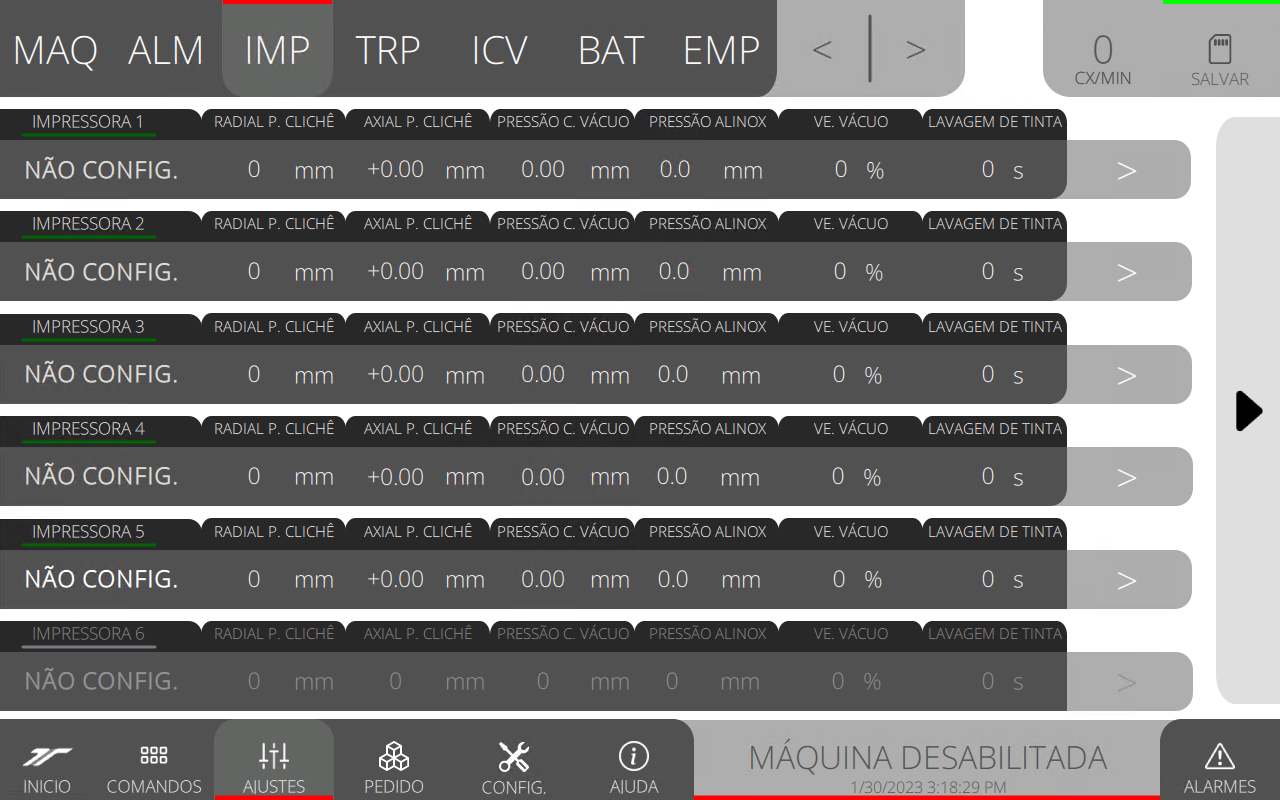
\includegraphics[width=480 px,height=300 px]{src/imagesICV/04-printters/01-printters/settings/e-Tela-Principal.png}
\end{figure}
\vspace*{\fill}

\newpage
\thispagestyle{fancy}
\vspace*{40 pt}
\subsubsection{\small{Vista geral dos ajustes das impressoras}} \label{sec:telaAjustesImpressorasVistaGeralAjustesImpressoras}
\vspace*{\fill}
\begin{figure}[h]
    \centering
    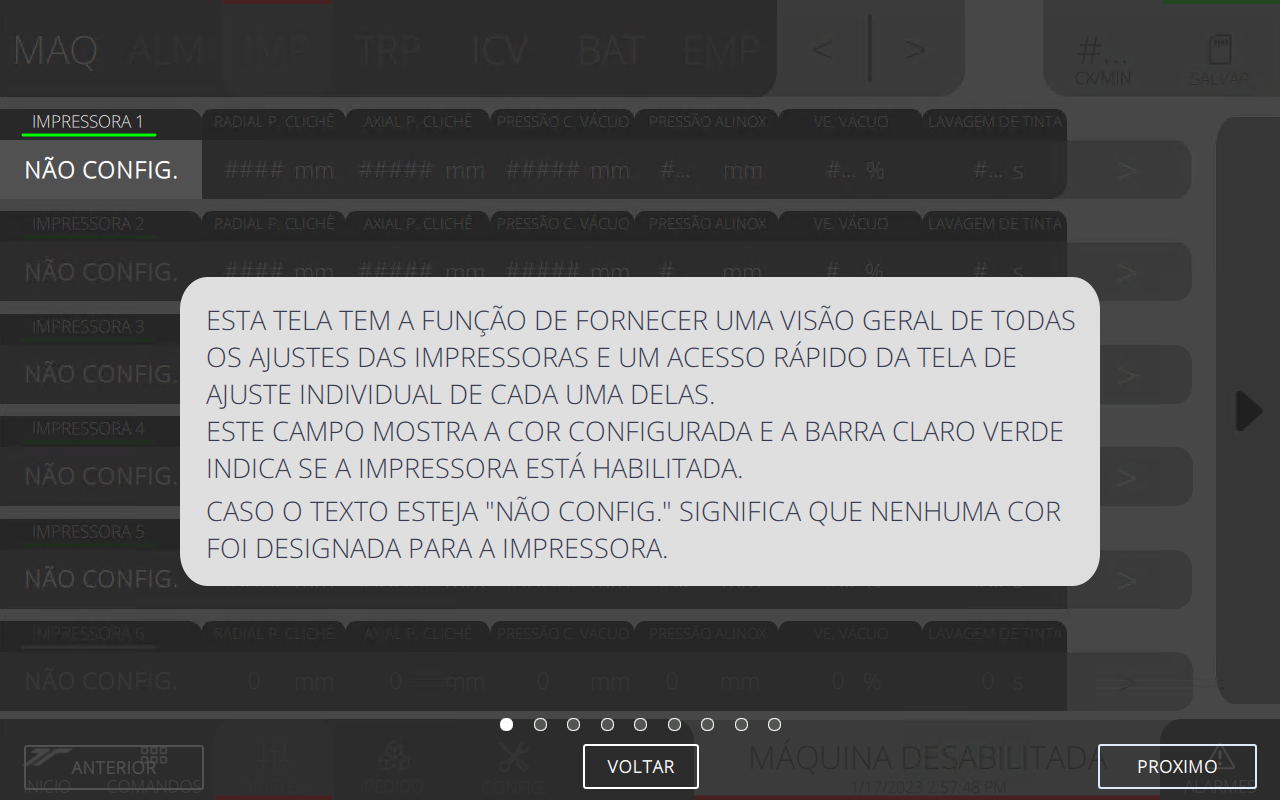
\includegraphics[width=576 px,height=360 px]{src/imagesICV/04-printters/01-printters/settings/1.png}
\end{figure}
\vspace*{\fill}

\newpage
\thispagestyle{fancy}
\vspace*{40 pt}
\subsubsection{\small{Aproximação do anilox bloqueada}} \label{sec:telaAjustesImpressorasAproximacaoAniloxBloqueada}
\vspace*{\fill}
\begin{figure}[h]
    \centering
    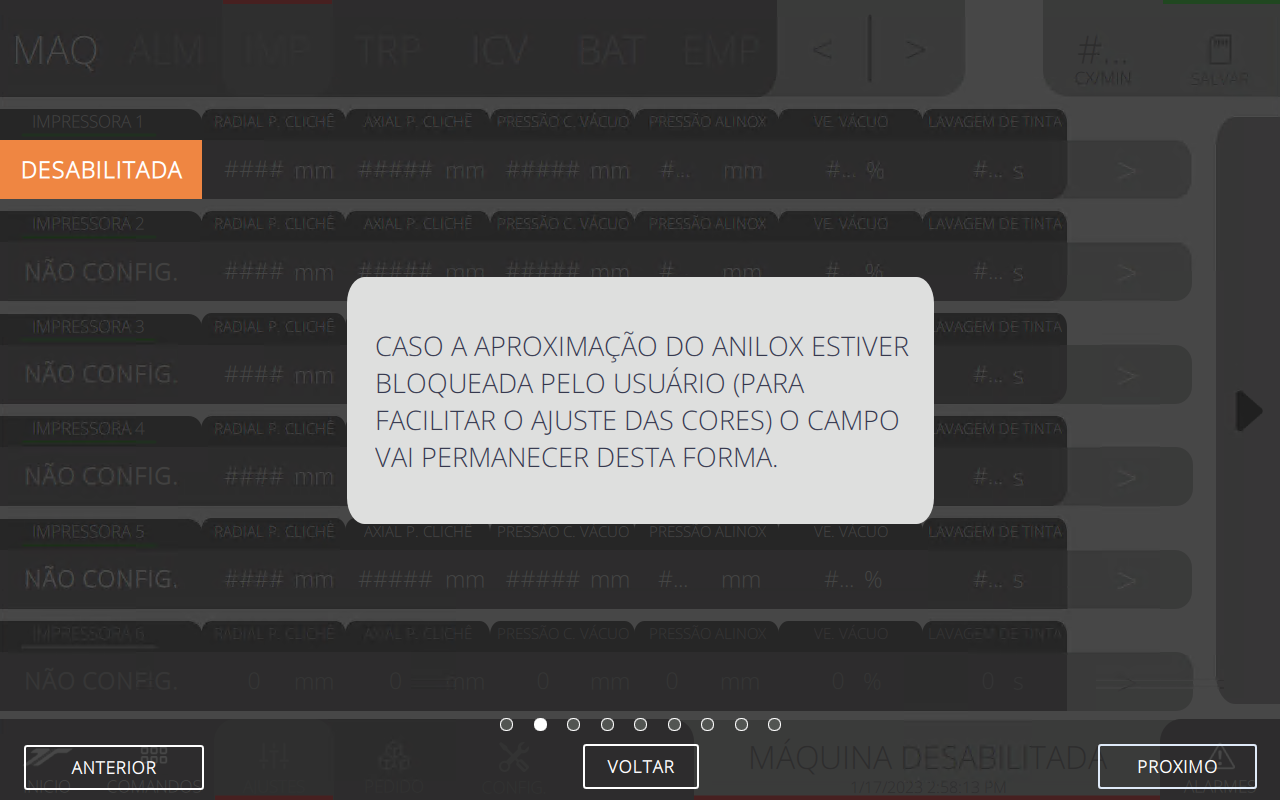
\includegraphics[width=576 px,height=360 px]{src/imagesICV/04-printters/01-printters/settings/2.png}
\end{figure}
\vspace*{\fill}

\newpage
\thispagestyle{fancy}
\vspace*{40 pt}
\subsubsection{\small{Registro atual}} \label{sec:telaAjustesImpressorasRegistroAtual}
\vspace*{\fill}
\begin{figure}[h]
    \centering
    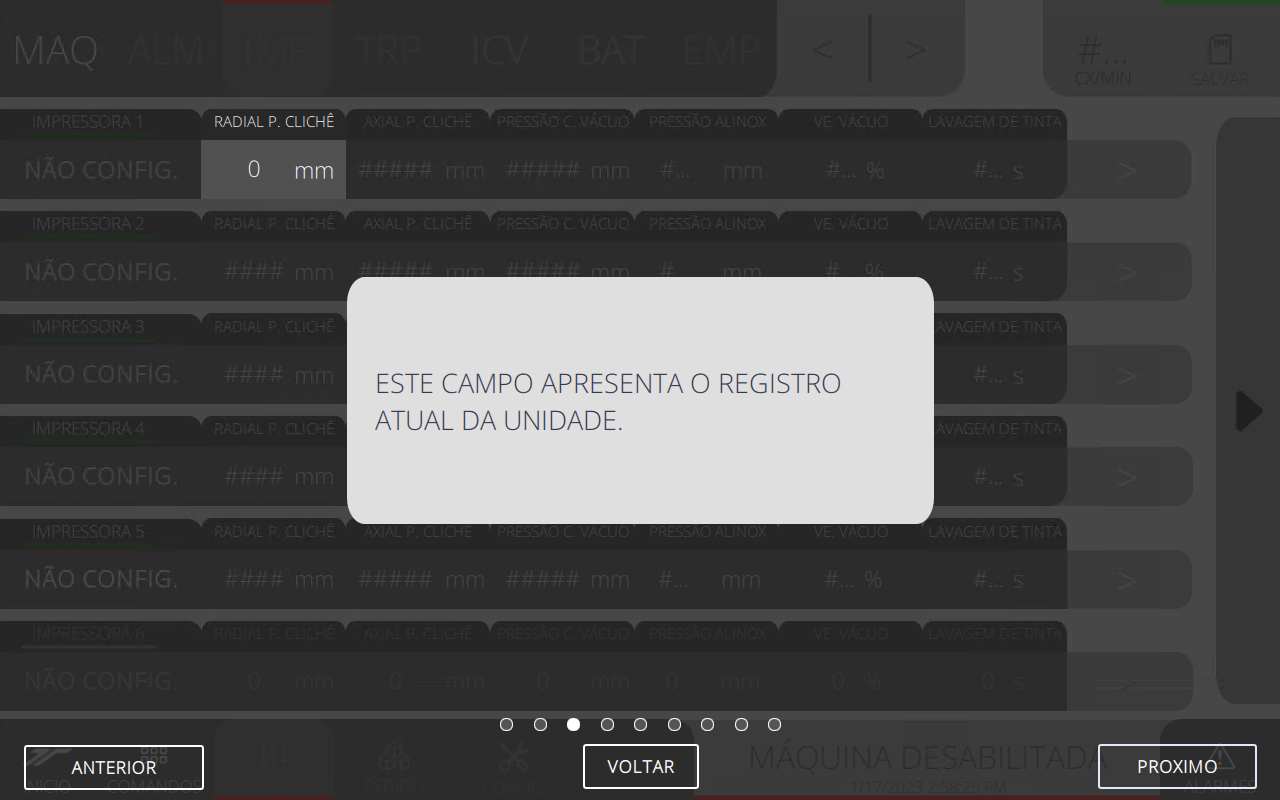
\includegraphics[width=576 px,height=360 px]{src/imagesICV/04-printters/01-printters/settings/3.png}
\end{figure}
\vspace*{\fill}

\newpage
\thispagestyle{fancy}
\vspace*{40 pt}
\subsubsection{\small{Ajuste axial do Clichê}} \label{sec:telaAjustesImpressorasAjusteAxialCliche}
\vspace*{\fill}
\begin{figure}[h]
    \centering
    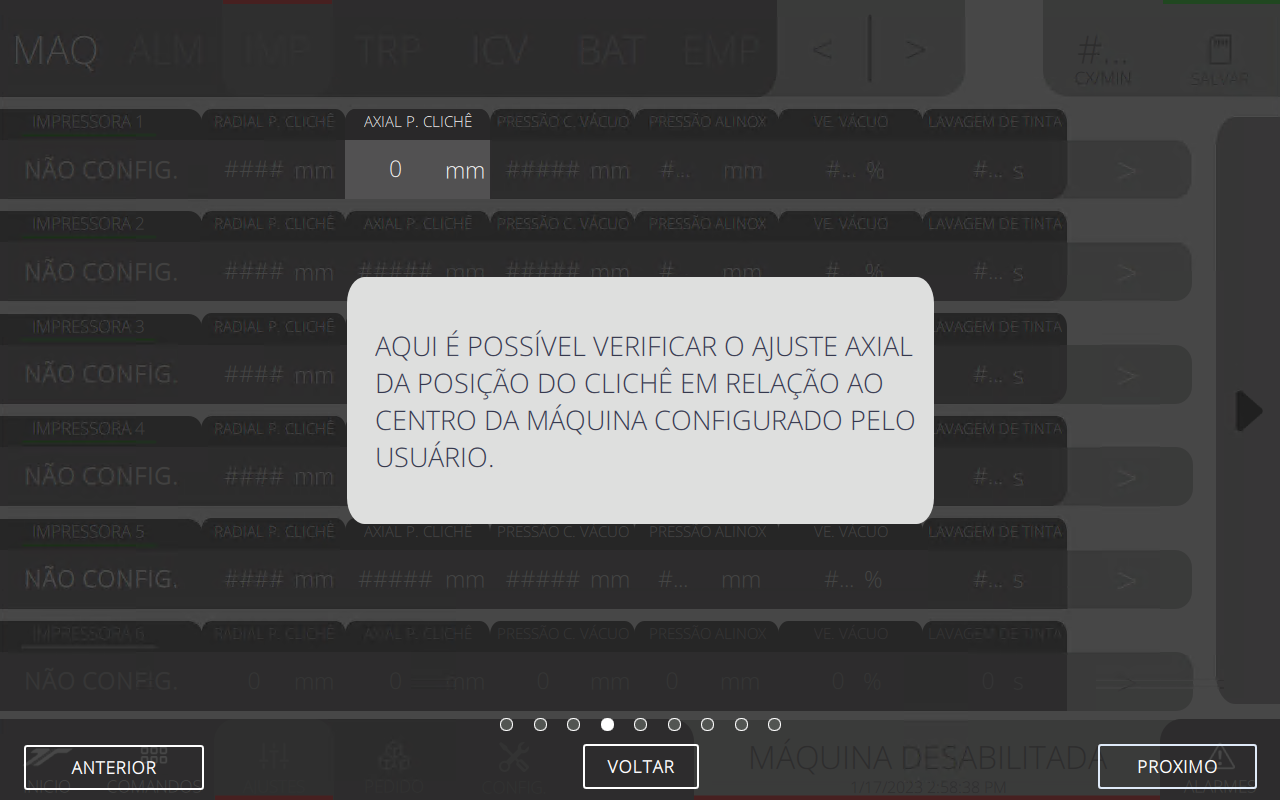
\includegraphics[width=576 px,height=360 px]{src/imagesICV/04-printters/01-printters/settings/4.png}
\end{figure}
\vspace*{\fill}

\newpage
\thispagestyle{fancy}
\vspace*{40 pt}
\subsubsection{\small{Pressão caixa de vácuo}} \label{sec:telaAjustesImpressorasPressaoCaixaVaco}
\vspace*{\fill}
\begin{figure}[h]
    \centering
    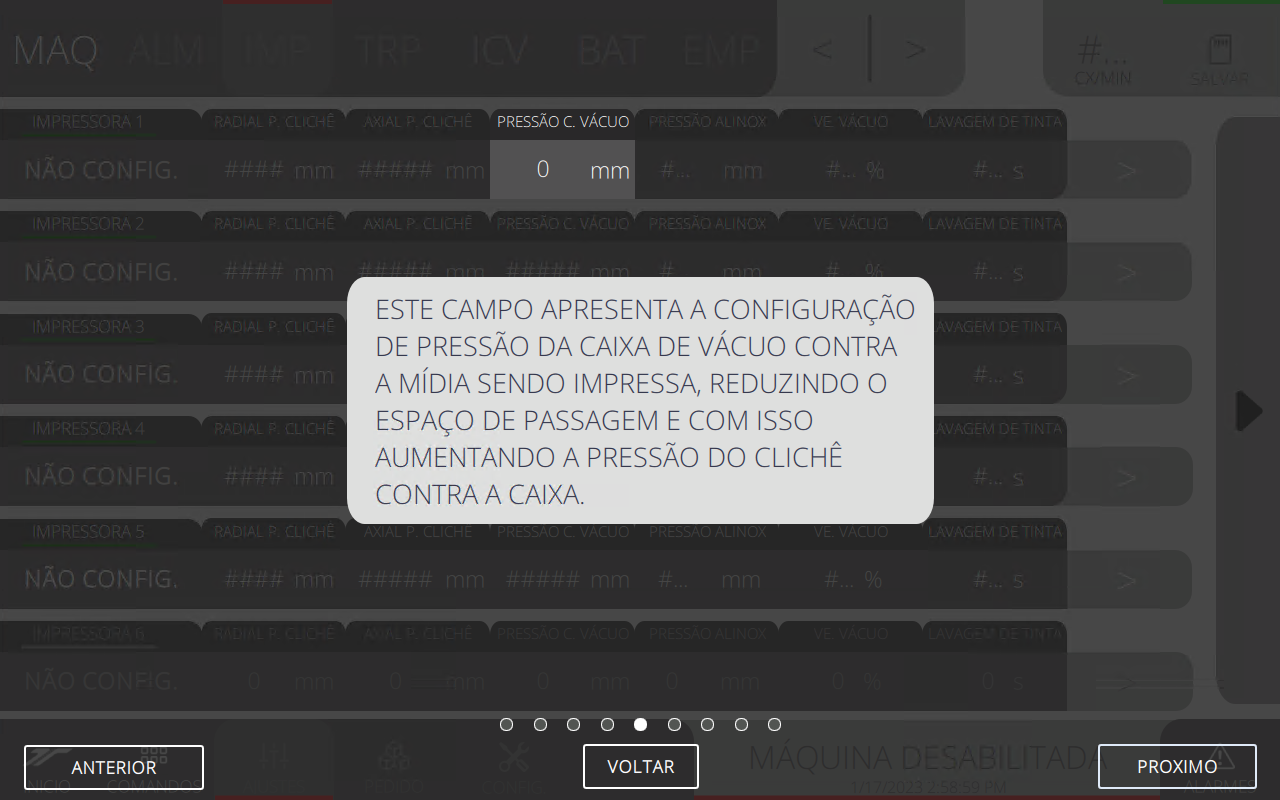
\includegraphics[width=576 px,height=360 px]{src/imagesICV/04-printters/01-printters/settings/5.png}
\end{figure}
\vspace*{\fill}

\newpage
\thispagestyle{fancy}
\vspace*{40 pt}
\subsubsection{\small{Pressão anilox}} \label{sec:telaAjustesImpressorasPressaoAnilox}
\vspace*{\fill}
\begin{figure}[h]
    \centering
    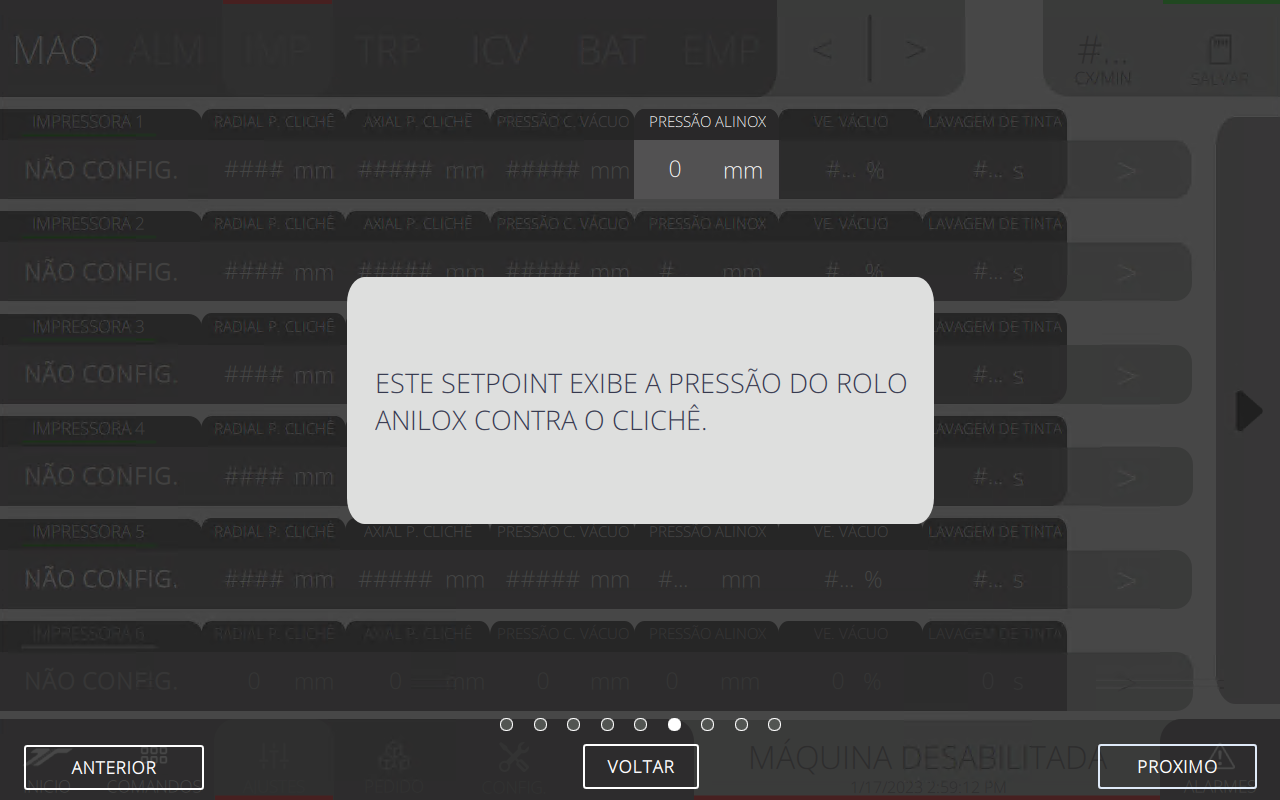
\includegraphics[width=576 px,height=360 px]{src/imagesICV/04-printters/01-printters/settings/6.png}
\end{figure}
\vspace*{\fill}

\newpage
\thispagestyle{fancy}
\vspace*{40 pt}
\subsubsection{\small{Intensidade do vácuo}} \label{sec:telaAjustesImpressorasIntensidadeVaco}
\vspace*{\fill}
\begin{figure}[h]
    \centering
    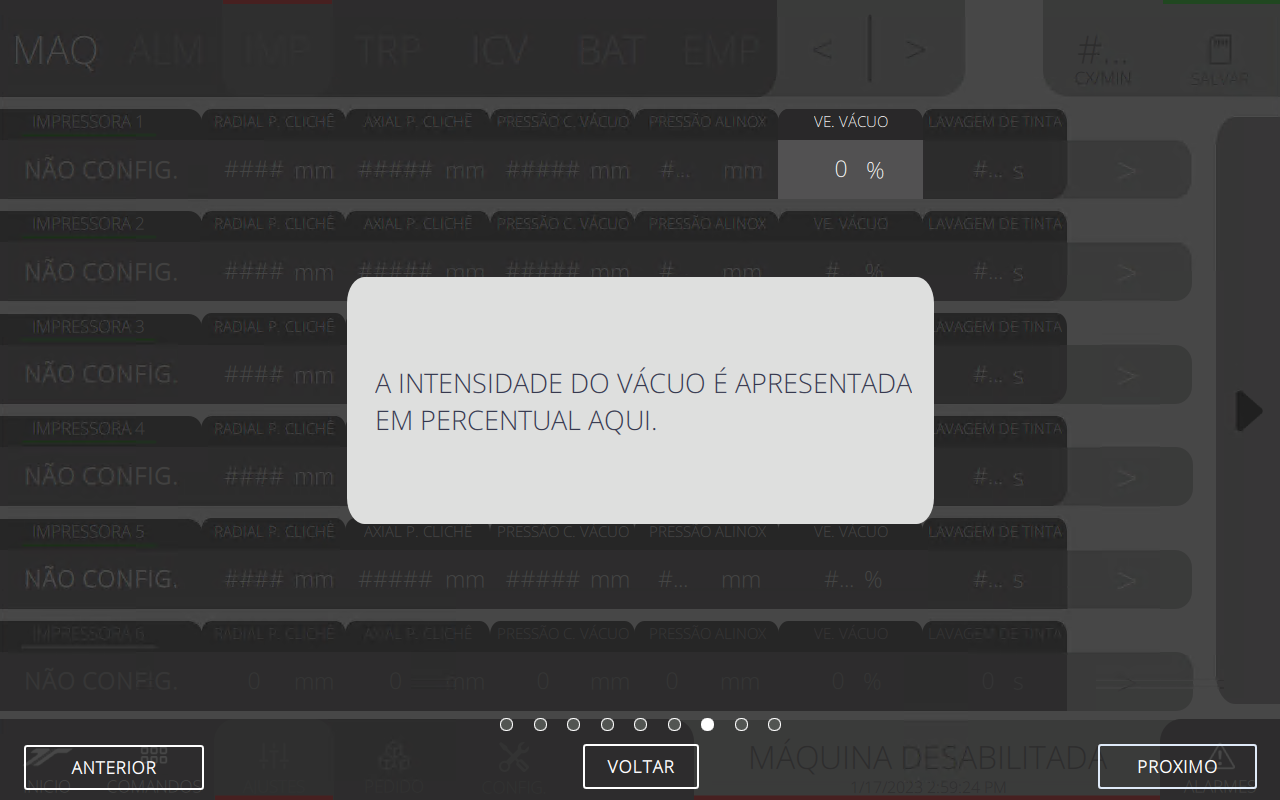
\includegraphics[width=576 px,height=360 px]{src/imagesICV/04-printters/01-printters/settings/7.png}
\end{figure}
\vspace*{\fill}

\newpage
\thispagestyle{fancy}
\vspace*{40 pt}
\subsubsection{\small{Tempo ativo da lavagem de tinta}} \label{sec:telaAjustesImpressorasTempoAtivoLavagemTinta}
\vspace*{\fill}
\begin{figure}[h]
    \centering
    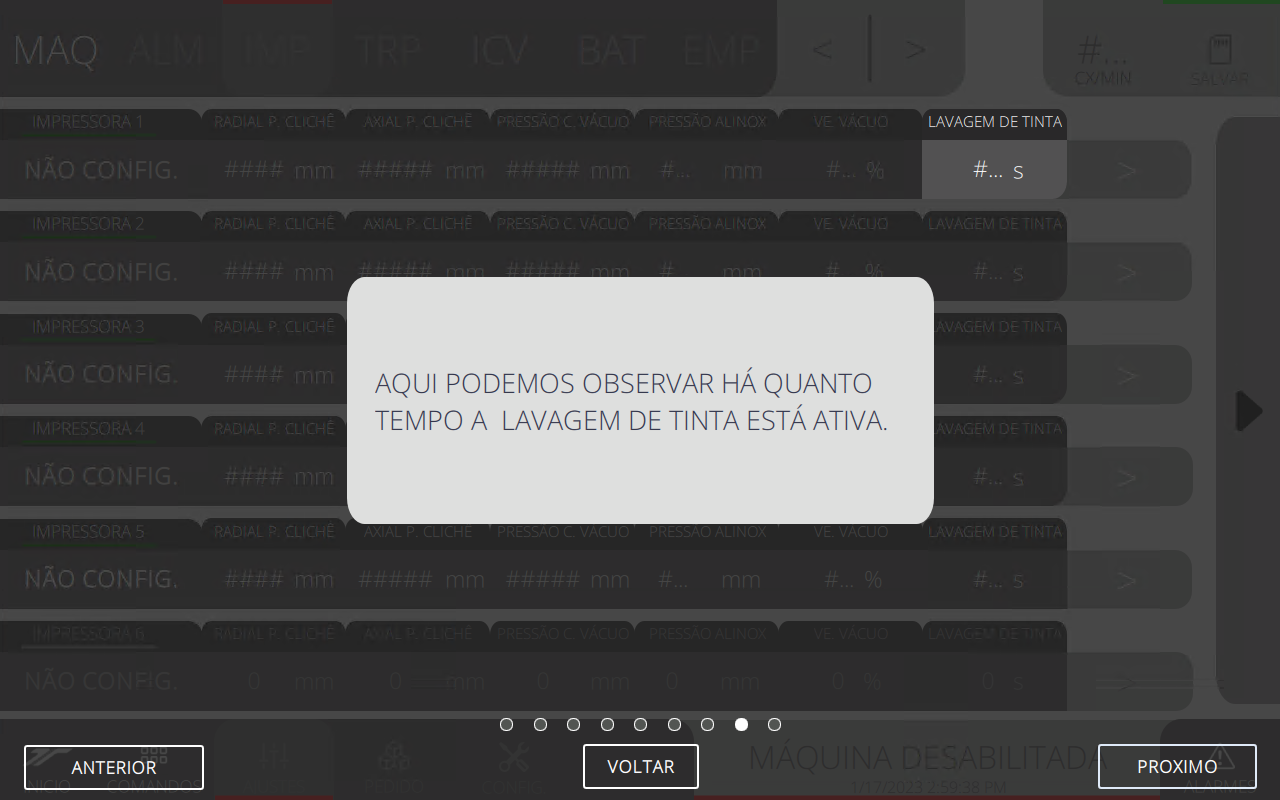
\includegraphics[width=576 px,height=360 px]{src/imagesICV/04-printters/01-printters/settings/8.png}
\end{figure}
\vspace*{\fill}

\newpage
\thispagestyle{fancy}
\vspace*{40 pt}
\subsubsection{\small{Ajuste individual da unidade}} \label{sec:telaAjustesImpressorasAjusteIndividualUnidade}
\vspace*{\fill}
\begin{figure}[h]
    \centering
    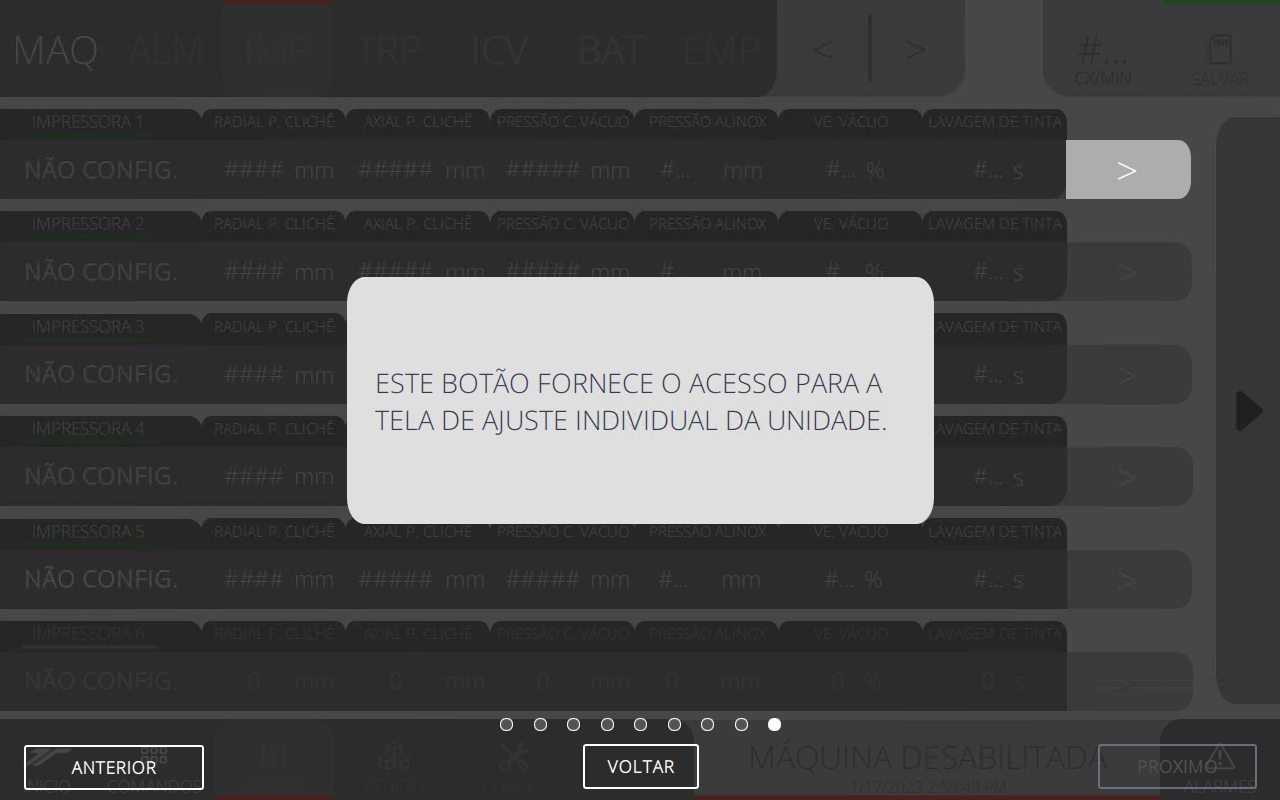
\includegraphics[width=576 px,height=360 px]{src/imagesICV/04-printters/01-printters/settings/9.png}
\end{figure}
\vspace*{\fill}

\newpage
\thispagestyle{fancy}
\vspace*{40 pt}
\subsection{Segunda tela geral dos ajustes das impressoras} \label{sec:segundaTelaGeralAjustesImpressoras}
Esta tela é acessada pelo botão direito "\textgreater" na tela de ajustes de \textbf{impressoras}. A lógica dos outros menus continua sendo a mesma da sua tela "pai" e para voltar a tela anterior basta clicar no botão esquerdo "\textless{}".
\vspace*{\fill}
\begin{figure}[h]
    \centering
    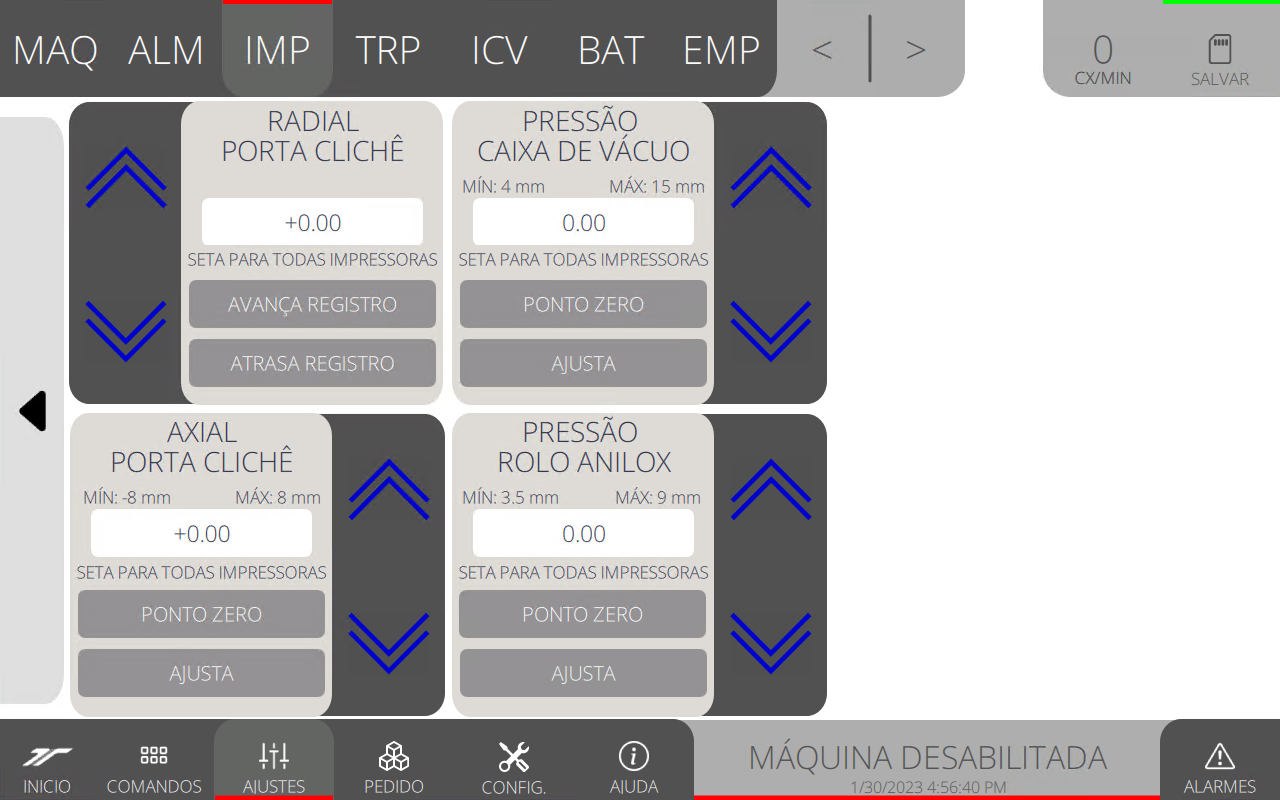
\includegraphics[width=480 px,height=300 px]{src/imagesICV/04-printters/01-printters/settings/e-Tela-Principal-2.png}
\end{figure}
\vspace*{\fill}

\newpage
\thispagestyle{fancy}
\vspace*{40 pt}
\subsubsection{\small{Axial porta clichê}}
\vspace*{\fill}
\begin{figure}[h]
    \centering
    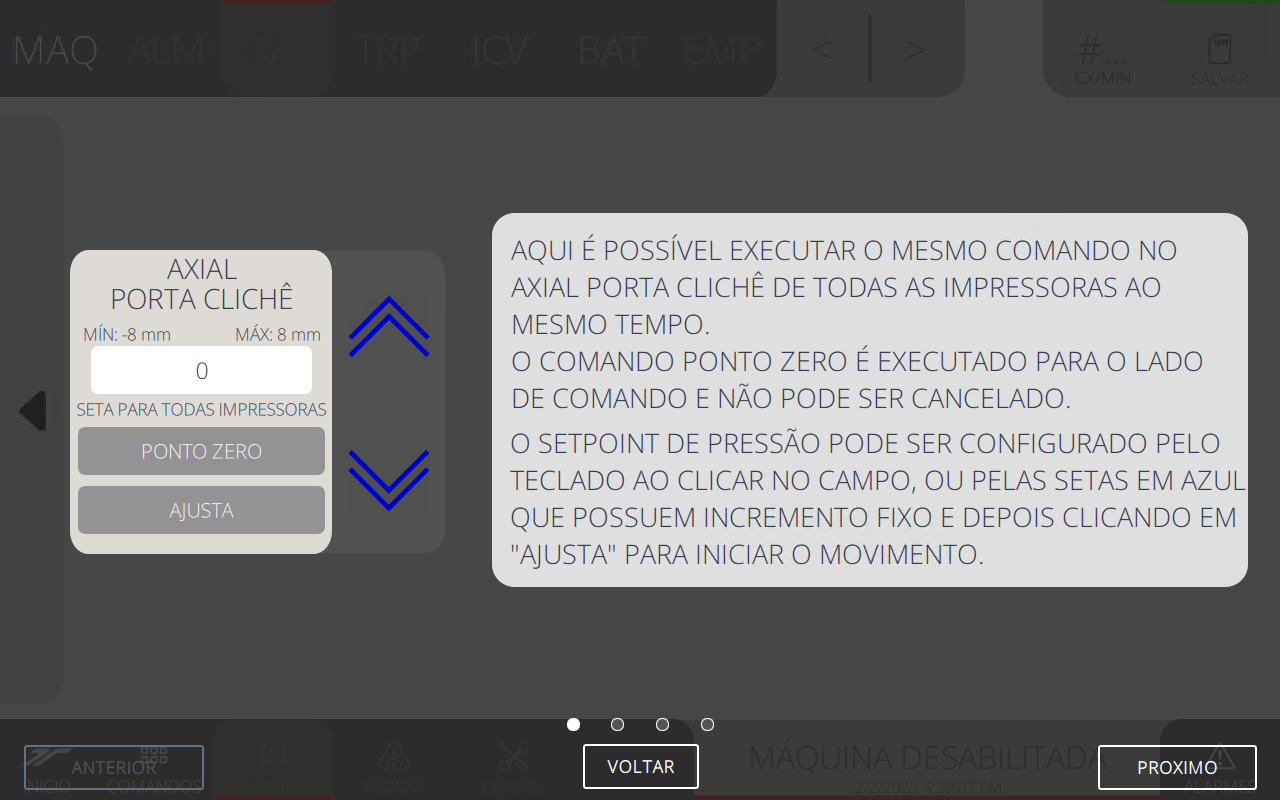
\includegraphics[width=576 px,height=360 px]{src/imagesICV/04-printters/01-printters/settings/10.png}
\end{figure}
\vspace*{\fill}

\newpage
\thispagestyle{fancy}
\vspace*{40 pt}
\subsubsection{\small{Pressão caixa de vácuo}} \label{sec:segundaTelaGeralAjustesImpressorasPressaoCaixaVaco}
\vspace*{\fill}
\begin{figure}[h]
    \centering
    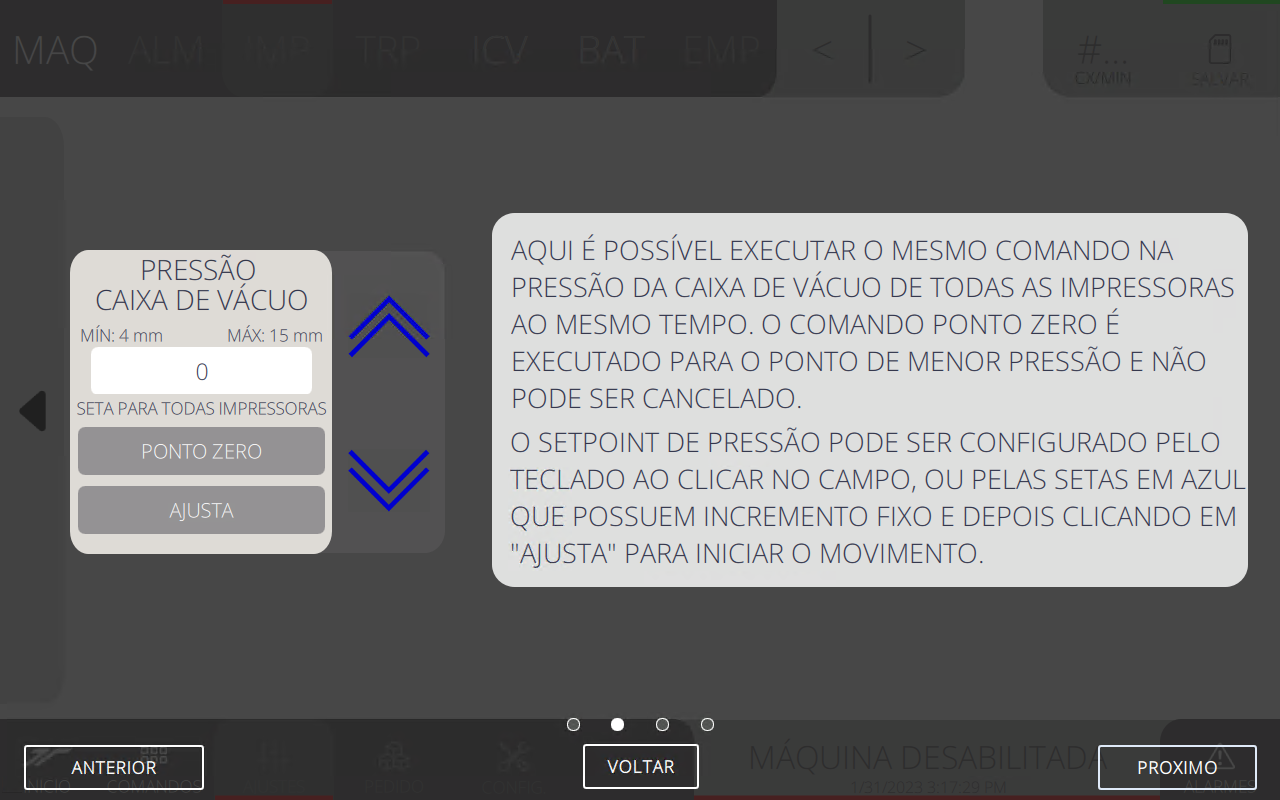
\includegraphics[width=576 px,height=360 px]{src/imagesICV/04-printters/01-printters/settings/11.png}
\end{figure}
\vspace*{\fill}

\newpage
\thispagestyle{fancy}
\vspace*{40 pt}
\subsubsection{\small{Radial porta clichê}} \label{sec:segundaTelaGeralAjustesImpressorasRadialPortaCliche}
\vspace*{\fill}
\begin{figure}[h]
    \centering
    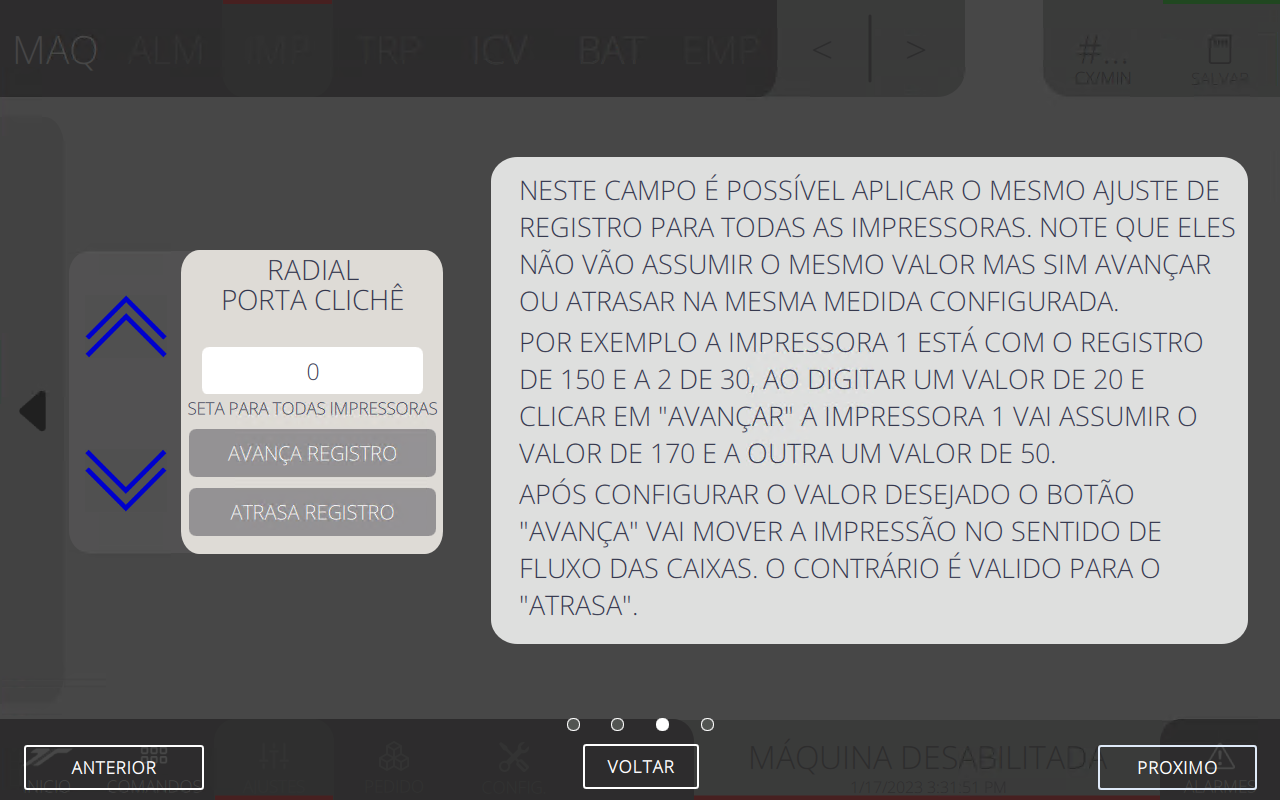
\includegraphics[width=576 px,height=360 px]{src/imagesICV/04-printters/01-printters/settings/12.png}
\end{figure}
\vspace*{\fill}

\newpage
\thispagestyle{fancy}
\vspace*{40 pt}
\subsubsection{\small{Pressão rolo anilox}} \label{sec:segundaTelaGeralAjustesImpressorasPressaoRoloAnilox}
\vspace*{\fill}
\begin{figure}[h]
    \centering
    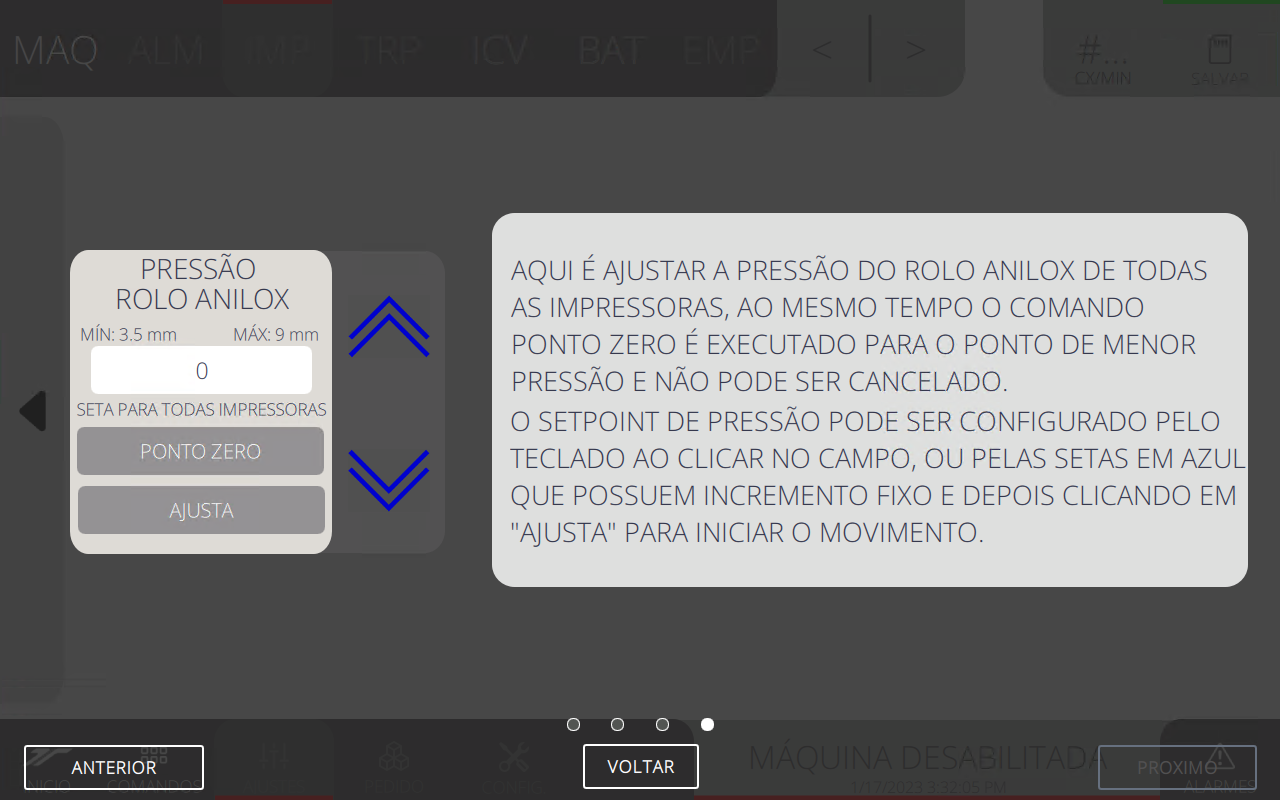
\includegraphics[width=576 px,height=360 px]{src/imagesICV/04-printters/01-printters/settings/13.png}
\end{figure}
\vspace*{\fill}